\scanpage{74}
\mspage{2}
\uline{Theorem} Let $S$ be an integral noetherian scheme, $X$ and $\unsure{\mathbb{X}|X}'$ proper over $S$ and $f:X'\quad X$ a surjective $S$-morphism, look at the corresponding homomorphisme for the Picard functors $f^{\bullet}:\text{\uuline{Pic}}_{X/S}\handwritten{\to}\text{\uuline{Pic}}_{X'/S}$. Assume: a) the existence problems A and B defined below for $X/S$ has always a solution (this is certainly true when $X/S$ is projective). b) the morphism $f_{s}:X'_{s}\handwritten{\to}X_{s}$ induced on the generic fiber is a morphism of descent,i.e. $\underline{O}_{X_{s}}\handwritten{\to}f(\underline{O}_{X'_{s}})=h(\underline{O}_{X''_{s}})$ is exact. Then, provided we replace $S$ by a suitable non empty open set, the homomorphism $f'$is representable by a quasi-affine morphism, more specifically \unsure{:|;} in the factorisation of $f^{\circ}$via the functor representing suitable descent data, $f^{\circ}=vu$ with $u$ affine and $v$ a monomorphism (as you well know), $v$ is in fact representable by \inserted{\handwritten{finite}} \unsure{divect|divest|divert|direct} sums of immersions.

\uline{Corollary} Without assuming b), but instead in a) allowing $X/S$ to be replaced by suitable other schemes $X_{i}$ finite over $X$, the same conclusion\deleted{s} \deleted{are} holds, namely $f^{\bullet}$is representable by quasi-affine morphisms.

This follows from the theorem, using a suitable factorisation of $f$. For instance, using Chow's lemma and the Main existence theorem in my first talk on Picard schemes, one gets:

\uline{Corollary 2} Assume $X/S$ proper satisfies the condition a') for every $X'$ finite over $X$, there exists a non empty open subset $S_{1}$ of $S$ such that problem A for $X'\quad S_{1}$ has allways solution \deleted{\unsure{of|for|on} problems A and B} (this condition is satisfied if $X/S$ is projective). Then provided we replace $S$ by a suitable $S_{1}$ non empty and open, $\underline{\mathrm{Pic}}_{X/S}$ exists, is separated, its connected components are of finite type over $S$.

\uline{N.B.} The proof does not give any evidence towards the fact that in
\margin{\handwritten{\figure{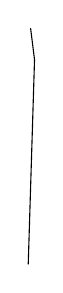
\begin{tikzpicture}\draw (0,0) -- (0.08,2.6) -- (0.03,3.0);\end{tikzpicture}}}}
the theorem, one could replace ``quasi-affine'' by ``affine''. This is true however over a field, bacause a quasi-affine algebraic group is affine ! It would be interesting to have a couterexample,say, over a ring of dimension $1$ such as $k\handwritten{[}t\handwritten{]}$\handwritten{,} $X$ and $X'$ projective and simple over $S$ and $X'\handwritten{\to}X$ birational, or alternatively, $X$ an\handwritten{d}$X'$ projective and normal over $S$, and $f:X'\handwritten{\to}X$ finite. A counterexample in the latter case would of course provide a counterrexample to the effectivity problem for a finite morphism raised in my first talk on descent ....

``Problem A'' is the following: given $X/S$ and Module $F$ on $X$, to represent the functor on the category of $S$-preschemes taking any $S'/S$ into a one-element or into the empty set, occording as to whether $F'$ on $X'/S'$ is flat with respect to $S'$ or not, where $X'=X\mathbin{x}_{S}S'$, $F'=F\mathbin{x}_{S}S'$.

\hfill .../...\par
% archive sheet number: 73
